\section{Code Examples}

\begin{frame}{Sorting}
    \begin{columns}
    \column{0.7\textwidth}
        \begin{itemize}
            \item percentageFullMatch = Percentage Full Match
            \item percentagePartialMatch = Percentage Partial Match
            \item getRating = Rating
            \item prevIngredients = Previous Ingredients
            \item recipe.Title = Recipe Title
        \end{itemize}
    \column{0.3\textwidth}
        \begin{figure}
            \centering
            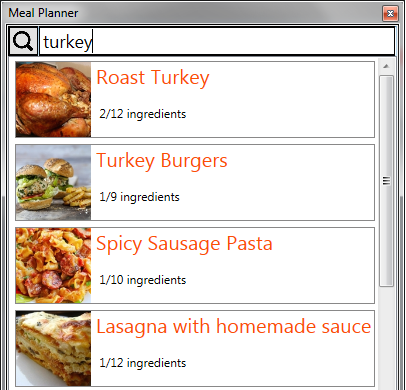
\includegraphics[width=\textwidth]{graphics/recipe-search-item}
        \end{figure}
    \end{columns}

\end{frame}

\begin{frame}{PublicQuerys}
    \begin{itemize}
        \item public IQueryable<inventoryListGroupedByQuantity> inventoryIQueryable
        \item public List<inventoryListGroupedByQuantity> inventoryList
        \item public List<LastMeal> ingredientsFromLastMeals
        \item public List<int> blackList
        \item public List<GrayList> grayList
    \end{itemize}
\end{frame}

\begin{frame}{Search by recipes}
    \begin{figure}
        \centering
        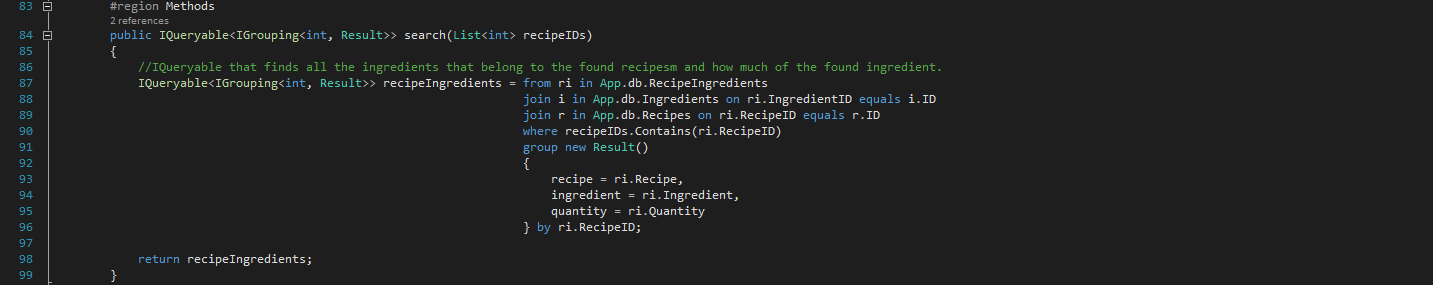
\includegraphics[width=\textwidth]{Grafik/search}
    \end{figure}
\end{frame}

\begin{frame}{Sorting of results}
    \begin{figure}
        \centering
        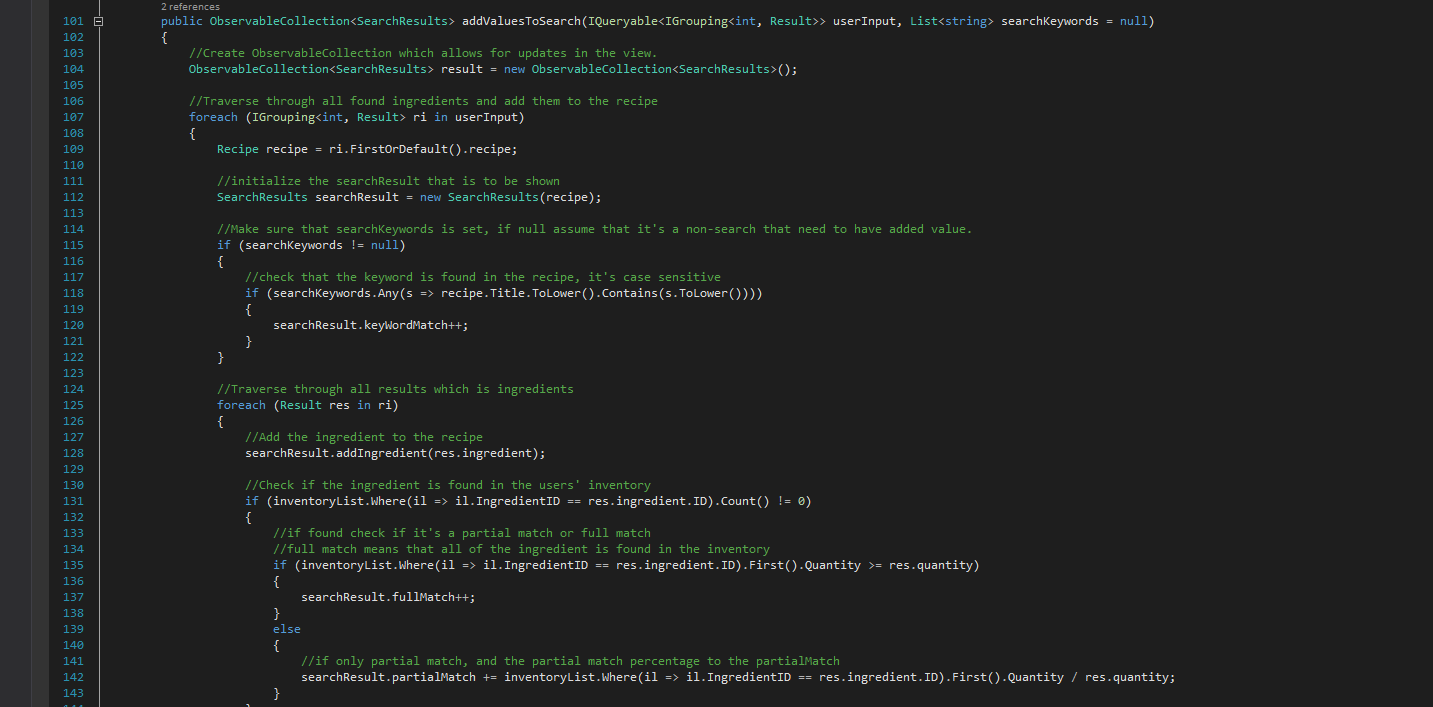
\includegraphics[width=\textwidth]{Grafik/sorter1}
    \end{figure}
\end{frame}
\begin{frame}{Sorting of results}
    \begin{figure}
        \centering
        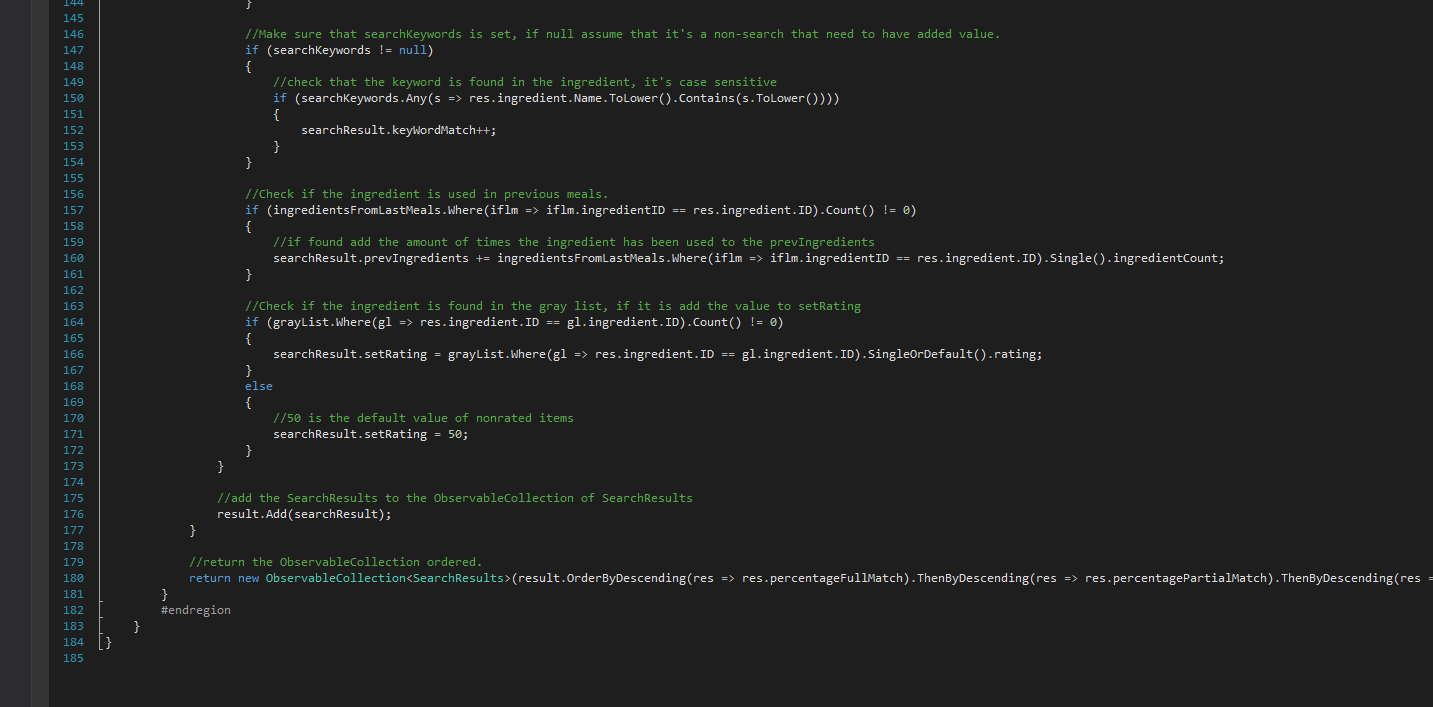
\includegraphics[width=\textwidth]{Grafik/sorter2}
    \end{figure}
\end{frame}




















